\documentclass[12pt,a4paper]{report}

\usepackage[a4paper,margin=2.5cm]{geometry}
\usepackage[T1]{fontenc}
\usepackage{newtxtext,newtxmath}
\usepackage[english]{babel}
\usepackage{setspace}
\usepackage{amsmath}
\usepackage{booktabs}
\usepackage{graphicx}
\usepackage{array}
\usepackage{tabularx}
\usepackage{adjustbox}
\usepackage{float}
\usepackage{xcolor}
\usepackage{tikz}
\usetikzlibrary{arrows.meta,positioning,calc}
\usepackage[authoryear,round]{natbib}
\usepackage{titlesec}
\usepackage[titles]{tocloft}
\usepackage[hidelinks]{hyperref}
\definecolor{ttblue}{HTML}{2A78D6}
\definecolor{ttorange}{HTML}{EB6834}
\definecolor{ttink}{HTML}{4D4C48}
\tikzset{
  ttbox/.style={draw=ttink, rounded corners=2pt, minimum height=7mm, minimum width=17mm, align=center, text=black},
  ttblue/.style={ttbox, draw=ttblue, fill=ttblue!14},
  ttorange/.style={ttbox, draw=ttorange, fill=ttorange!14},
  ttop/.style={circle, draw=ttink, fill=white, minimum size=6.5mm, inner sep=0pt, text=black},
  ttnote/.style={font=\scriptsize, text=ttink, align=center},
  ttarrow/.style={-{Stealth[length=2mm]}, line width=0.6pt, draw=ttink},
}

\usetikzlibrary{arrows.meta,positioning,fit,calc,decorations.pathreplacing}
\definecolor{cblue}{HTML}{2A78D6}\definecolor{cbluef}{HTML}{DBE8F8}
\definecolor{corange}{HTML}{EB6834}\definecolor{corangef}{HTML}{FBE1D6}
\definecolor{cink}{HTML}{4D4C48}
\tikzset{
  box/.style={draw=cink, rounded corners=2pt, align=center, minimum height=0.75cm, inner sep=3pt, font=\small},
  op/.style={draw=cink, circle, minimum size=0.6cm, inner sep=0pt, font=\small, fill=white},
  note/.style={font=\scriptsize, text=cink, align=center},
  flow/.style={-{Stealth[length=5pt]}, draw=cink, thick},
  carry/.style={-{Stealth[length=5pt]}, draw=corange, very thick},
}
\usetikzlibrary{arrows.meta,positioning,fit,calc,backgrounds}
\tikzset{ttcross/.style={draw=red!70!black, line width=1.3pt}}
\newcommand{\ttx}[1]{%
  \draw[ttcross] ($(#1)+(-0.22,-0.22)$) -- ($(#1)+(0.22,0.22)$);
  \draw[ttcross] ($(#1)+(-0.22,0.22)$) -- ($(#1)+(0.22,-0.22)$);}
% #1 = separate path A (1/0), #2 = trained through B (1/0), #3 = title, #4 = gains
\newcommand{\ablpanel}[4]{%
\begin{tikzpicture}[font=\small]
  \ifnum#1=1 \def\aop{1}\else\def\aop{0.25}\fi
  \ifnum#2=1 \def\bop{1}\else\def\bop{0.25}\fi
  \node[ttblue]   (Si) at (0,0)    {$S_{\mathrm{in}}$};
  \node[ttorange] (Sc) at (0,-1.4) {$S_{\mathrm{carried}}$};
  \node[ttop, draw=ttblue] (g) at (2.0,0) {$g$};
  \node[ttnote, above=1pt of g, text=ttblue] {bias $-6$};
  \node[ttop] (plus) at (5.4,0) {$+$};
  \draw[ttarrow] (Si.east) -- (g.west);
  \draw[ttarrow] (g.east) -- (plus.west);
  \draw[ttarrow] (plus.east) -- ++(0.6,0);
  \begin{scope}[opacity=\aop]
    \node[ttbox, draw=ttorange, minimum width=11mm] (clip) at (2.0,-1.4) {clip};
    \node[ttop, draw=ttorange] (gc) at (3.3,-1.4) {$g_c$};
    \node[ttop, draw=ttorange] (al) at (4.4,-1.4) {$\alpha$};
    \draw[ttarrow] (Sc.east) -- (clip.west);
    \draw[ttarrow] (clip.east) -- (gc.west);
    \draw[ttarrow] (gc.east) -- (al.west);
    \draw[ttarrow] (al.east) -| (plus.south);
  \end{scope}
  \ifnum#1=0
    \ttx{gc}
    \draw[ttarrow, draw=ttorange] (Sc.north) -- node[ttnote, right, text=ttorange] {seeds $S_{\mathrm{in}}$} (Si.south);
  \fi
  \begin{scope}[opacity=\bop]
    \draw[ttarrow, dashed] (4.4,-2.3) -| node[pos=0.25, below, ttnote] {gradient from the next slice} (Sc.south);
  \end{scope}
  \ifnum#2=0 \ttx{2.2,-2.3} \fi
  \node[font=\small\bfseries] at (2.7,-3.2) {#3};
  \node[ttnote] at (2.7,-3.6) {between slices: #4};
\end{tikzpicture}}

\newcommand{\sig}{$^{*}$}
\newcommand{\reporttitle}{Session-Persistent Test-Time Training for Language Models: Transfer and Interference of a Carried Fast Weight Across Documents}
\newcommand{\authorname}{M A S I Malimbada}
\newcommand{\regno}{KIC-BSCCSAI-25.1-P-014}
\newcommand{\affiliation}{Kandy Innovation Centre, National Institute of Business Management}
\newcommand{\authoremail}{suchitraidumina@gmail.com}
\newcommand{\submissiondate}{\rule{4cm}{0.4pt}}

\newcommand{\twodigit}[1]{\ifnum#1<10 0\fi\number#1}
\titleformat{\chapter}[display]{\normalfont\bfseries\Large}{Chapter \twodigit{\value{chapter}}:}{0.4em}{\LARGE}
\titlespacing*{\chapter}{0pt}{2.5em}{1.5em}
\usepackage{etoolbox}
\makeatletter
\patchcmd{\chapter}{\if@openright\cleardoublepage\else\clearpage\fi}{}{}{}
\makeatother
\titleformat{\section}{\normalfont\bfseries\large}{\thesection.}{1em}{}
\titleformat{\subsection}{\normalfont\bfseries\normalsize}{\thesubsection.}{1em}{}
\renewcommand{\contentsname}{Table of Contents}
\renewcommand{\bibname}{References}
\renewcommand{\cftchappresnum}{Chapter 0}
\renewcommand{\cftchapaftersnum}{:}
\setlength{\cftchapnumwidth}{6.2em}
\renewcommand{\cftsecaftersnum}{.}
\renewcommand{\cftsubsecaftersnum}{.}
\renewcommand{\cfttabpresnum}{Table }
\renewcommand{\cfttabaftersnum}{:}
\setlength{\cfttabnumwidth}{5.8em}
\renewcommand{\cftfigpresnum}{Figure }
\renewcommand{\cftfigaftersnum}{:}
\setlength{\cftfignumwidth}{6.4em}

\begin{document}

\begin{titlepage}
\centering
\vspace*{1cm}

{\bfseries\Large KANDY INNOVATION CENTRE\par}
\vspace{0.3cm}

{\bfseries\Large NATIONAL INSTITUTE OF BUSINESS MANAGEMENT\par}
\vspace{0.3cm}

{\bfseries\large BACHELOR OF SCIENCE IN COMPUTER SCIENCE WITH AI\par}

\vspace{2.5cm}

{\Large Individual Project Report\par}

\vspace{2.5cm}

{\LARGE\bfseries \reporttitle\par}

\vspace{3cm}

{\large The Assignment Submitted by\par}
\vspace{0.4cm}

{\large\bfseries \authorname\par}
{\large (\regno)\par}

\vfill

{\large \today\par}

\end{titlepage}
\pagenumbering{roman}
\setcounter{page}{2}

\chapter*{Abstract}
\phantomsection
\addcontentsline{toc}{chapter}{Abstract}

\begin{center}
{\bfseries \reporttitle\par}
\vspace{0.3cm}
\authorname\par
\affiliation\par
\authoremail\par
\end{center}
\vspace{0.3cm}

Test-time training (TTT) in the context of large language models adapts a set of fast weights during inference, but most existing methods discard them at the document boundary. In this research we study what happens when the fast weights are carried into the next document, using SlimPajama-6B and English Wikipedia. Building on In-Place TTT in Qwen3-0.6B, we introduce a gated carry, in which the state of previous text is carried through a separate, zero-initialised gated path trained by backpropagation across slice boundaries. Compared with resetting the state, the gated carry lowers perplexity on the continuation of a document by about 1\% when the earlier text is no longer in the attention context. Across documents, we found that its effect depends on how much those documents relate, and that it raises perplexity after text from another source and, in a chain of development documents from the same source at step 600, after those documents too. Most of the gain is a generic effect of the source, but a related article still outperforms a carry averaged over 200 articles. Training across document boundaries removes the harm after text from another source and, with it, this advantage of related text, and it lowers the gain within a document.

\clearpage
\phantomsection
\addcontentsline{toc}{chapter}{Table of Contents}
\tableofcontents
\clearpage
\phantomsection
\addcontentsline{toc}{chapter}{List of Tables}
\listoftables
\clearpage
\phantomsection
\addcontentsline{toc}{chapter}{List of Figures}
\listoffigures

\clearpage
\pagenumbering{arabic}

% ======================================================================
\chapter{INTRODUCTION}

A language model adapts to its input through attention. Therefore, the information it gains from its context is lost when a new session starts. Test-time training (TTT) offers a partial solution to this issue. In TTT, some model weights get updated during inference. In-Place TTT \citep{feng2026inplace} does this by updating $W_{\mathrm{down}}$ inside MLP blocks of an existing transformer. Most such methods, however, reset their fast weights at the end of each document \citep{sun2025learning,tandon2025endtoend,feng2026inplace}. In this research, we ask whether a fast weight built on one document helps or harms the next, and on what this depends.

\section{Background of the study}

Test-time training updates part of a model on the input it is currently reading, with a self-supervised objective~\citep{sun2020ttt}. When it comes to language models, it has been used to build sequence layers whose hidden state is a small model trained online \citep{sun2025learning}, memory modules beside attention \citep{behrouz2025titans}, and In-Place TTT \citep{feng2026inplace}, which turns the MLP down-projection of a pretrained transformer into a fast weight. These weights change during inference and act as an associative memory of recent input \citep{hinton1987using,schmidhuber1992learning,ba2016using,schlag2021linear}.

\section{Justification of the problem}

In-Place TTT resets its fast weights at document boundaries to prevent leakage between unrelated inputs. It therefore does not test carrying them forward \citep{feng2026inplace}. According to other research, it is not obvious whether carrying the weights helps. Selective state-space models can pass or reset their state at a boundary \citep{gu2024mamba}. Dynamic evaluation carries gradient updates of the slow weights along a test stream and benefits from it \citep{krause2018dynamic}. In pretraining, earlier documents in the attention context help when they are related and distract when they are not \citep{zhao2024analysing}. Therefore, a carried fast weight can help or interfere with the model's performance. To our knowledge, no work has given a TTT fast weight a trained carry path and measured how its effect depends on the relation between consecutive documents.

\section{Objectives of the study}

The study addresses two research questions.
\begin{description}
  \item[Q1.] How much does the carry contribute to language modelling?
  \item[Q2.] Which domains benefit most from session-persistent TTT?
\end{description}
We answer them in perplexity on held-out text, which measures stream and domain adaptation in the sense of \citet{song2026beyond}. In this research, we do not make any claims that carried state stores information that the model can later retrieve. Our contributions are as follows.
\begin{itemize}
  \item We introduce a gated carry, which passes the fast weight from earlier text to later text using a gated path. The path starts switched off and is trained using backpropagation. Compared with resetting the fast weight, it lowers perplexity on the rest of a document by about 1\% when the earlier slices are not in the attention context, at two training seeds (Section~\ref{sec-within}).
  \item We show that, across documents, the carry's effect depends on how related the earlier text is. We found that it helps most after the target's own opening, less after a related article and less again after an unrelated one, and it raises perplexity after text from another source. This pattern is the same at both seeds. Most of the gain comes from having read text of the same source, and only a small part from the specific related article (Section~\ref{sec-transfer}).
  \item At two seeds (the second not preregistered), training the carry across document boundaries stops text from another source from harming perplexity (same-source chains were not tested). But, a related article then no longer beats a generic carry, and the gain between slices of a document falls (Section~\ref{sec-across}).
\item Most of the lead of the gated carry over a LoRA-only model comes from its extra trainable parameters. Against a single-seed control with the same architecture and parameters but no fast-weight updates, the gated carry still lowers perplexity by 0.07 to 0.10 (Section~\ref{sec-compare}).
\item Within a document, placing the earlier text in the attention context lowers perplexity about 25 times more than the carry does. Therefore, the carry's possible value lies where that text is no longer in context (Section~\ref{sec-compare}).
\end{itemize}

% ======================================================================
\chapter{LITERATURE REVIEW}

\section{Test-time training}

\citet{sun2020ttt} introduced test-time training for image classification. In it, a shared feature extractor is adapted on a self-supervised loss of each test input and reset before the next, although an online variant keeps the update across a stream of test inputs. Later work kept the reset and showed that a misaligned signal can lower accuracy \citep{gandelsman2022ttt}, while online test-time adaptation keeps its updates across test batches \citep{wang2021tent}, and continual test-time adaptation must then limit forgetting and accumulated error \citep{wang2022cotta,maharana2026continual}. In language models, TTT layers restart from a learned state for every sequence \citep{sun2025learning}, and end-to-end TTT discards short training documents to avoid resetting at packed boundaries \citep{tandon2025endtoend}. In-Place TTT applies the current fast weight to each chunk, then adds an outer product of a target and the MLP activation, and resets at document boundaries \citep{feng2026inplace}. Under matched training its original target does not improve long-context retrieval, while a next-position target does \citep{ouyang2026ttt}. Other work trains test-time memory for a later use, by distilling a long-context teacher into the fast weights \citep{wang2026learning} or by supervising a question asked long after the facts were read \citep{kim2026delayed}, both within one context.

\section{Fast weights, update rules and stability}

Causal linear attention is a recurrent network whose state adds the outer product of each key and value \citep{katharopoulos2020transformers}, and this state is a fast-weight matrix \citep{schlag2021linear}. An additive, or Hebbian, state cannot easily overwrite a stale association and holds without interference at most as many associations as its key dimension \citep{schlag2021linear,yang2024deltanet}. The delta rule \citep{widrow1960adaptive} writes the prediction error. Which is equal to one step of online gradient descent \citep{yang2024deltanet}, and the rule lowers WikiText-103 test perplexity by 1.5 to 2.8 points at matched size \citep{schlag2021linear}. Gates and decays let a state forget \citep{ba2016using,mao2022finetuning,yang2025gated}, and in a controlled ablation linear attention without a gate trains markedly worse than with one \citep{yang2024gla}. Every family needs a mechanism that keeps its state in range, such as normalisation \citep{zhang2025test}, decay \citep{ba2016using} or, in one evaluation of In-Place TTT, an inference-time clip on each update \citep{feng2026inplace}. A norm bound applied to a large state keeps only its direction.

\section{Persistence across documents}

Most memory architectures persist within one stream. Transformer-XL caches the activations of the previous segment \citep{dai2019transformerxl}, the Recurrent Memory Transformer passes memory tokens that are trained through several segments \citep{bulatov2022rmt}, and Memorizing Transformers clear their memory at each new document \citep{wu2022memorizing}. Compressive memories keep a summary of earlier segments \citep{rae2019compressive,munkhdalai2024leave}. \citet{schlag2021linear} carry the state across training segments, where the additive rule breaks down with perplexity above 260, and recurrent models whose state is passed on from a different sequence during training generalise to longer inputs \citep{buitrago2025understanding}. Fast-weight product key memory keeps its fast weights across segments, and when it reads several domains in turn, the newer domains replace the gains of the earlier ones \citep{zhao2026fwpkm}. Adapting a language model to the recent text of a stream predates neural models \citep{kneser1993dynamic}. Dynamic evaluation persists across texts by gradient steps on the slow weights, and its gain levels off within a few thousand characters of in-distribution text \citep{krause2018dynamic}. Memory can also persist in an external episodic memory \citep{das2024larimar} or in the parameters, as a self-updated memory pool \citep{wang2024memoryllm}, a compact key-value cache distilled from a corpus before deployment \citep{eyuboglu2025cartridges}, or by writing facts into the weights one after another, which forgets earlier facts \citep{oneill2026continually}, and lifelong in-context learning has been argued to require such parametric state \citep{mcdermott2026lifelong}. Test-time training on retrieved neighbours helps, and training from the nearest to the farthest neighbour works better than the reverse \citep{hardt2024test}. Therefore, transfer is expected to follow relatedness.

\section{Evaluation methodology and research gap}

Perplexity is the standard measure in this literature \citep{meister2021beyond}, but with large samples almost any difference is significant. Therefore, we report effect sizes with intervals. \citet{song2026beyond} separate stream and domain adaptation, which perplexity supports, from claims of memory, which need behavioural tests, and place In-Place TTT at the first level. The gap we address is therefore specific. To our knowledge, no prior work gives a TTT fast weight a trained carry path, measures it against a reset at the document boundary, and asks how its effect depends on the relatedness of the earlier text.

% ======================================================================
\chapter{METHODOLOGY}

We extend a pretrained language model with In-Place TTT layers and a gated carry, train it alongside a matched control, and compare the two on held-out text under paired evaluation conditions that isolate each source of gain. It is implemented in Python with PyTorch \citep{paszke2019pytorch}, Hugging Face Transformers \citep{wolf2020transformers} and PEFT \citep{mangrulkar2022peft}, and the models are trained and evaluated on cloud GPUs.

\section{Data Collection}

Training and the main evaluation use the SlimPajama-6B subset \citep{yoon2023slimpajama6b} of SlimPajama \citep{soboleva2023slimpajama}, a cleaned and deduplicated derivative of RedPajama~\citep{weber2024redpajama}. It has seven sources. We drop CommonCrawl, which is about 54\% of the data, and use the other six, which are ArXiv, Book, C4, Github, StackExchange and Wikipedia (Table~\ref{tab-data}). Transfer between related documents is measured on English Wikipedia articles from the November 2023 dump \citep{wikimedia2023wikipedia}. We use the titles mentioned in one article to link it to another.

\begin{table}[H]
  \centering
  \small
  \begin{tabularx}{\linewidth}{>{\raggedright\arraybackslash}p{4cm}>{\raggedright\arraybackslash}X>{\raggedright\arraybackslash}p{3.4cm}}
    \toprule
    Data & Content & Use \\
    \midrule
    SlimPajama-6B, training & 4000 documents of 2048 to 16{,}384 tokens & training \\
    SlimPajama-6B, development holdout & 106 documents, 656{,}331 tokens & development evaluation \\
    SlimPajama-6B, confirmatory holdout & 73 further documents & confirmatory evaluation \\
    Wikipedia, shards 0 and 1 & 200 target articles with primes & development relatedness \\
    Wikipedia, shards 2 and 3 & 200 target articles with primes, 200 articles for a generic carry, 10 chain articles per target & confirmatory relatedness \\
    \bottomrule
  \end{tabularx}
   \caption{Outline of the data.}
  \label{tab-data}
\end{table}

\section{Data Preprocessing}

Training documents are balanced towards 25\% C4, 20\% each of Github and ArXiv, 15\% Book and 10\% each of Wikipedia and StackExchange. If a document is shorter than 2100 tokens, it is read as one document. If not, it is split into two to six slices where each slice is at least 1000 tokens. Held-out documents come from the last 15{,}000 rows of the dataset, and they are removed before training. Wikipedia articles of at least 12{,}000 characters serve as targets and those of at least 6{,}000 characters as primes. Every prime and scored text is a block of 1024 tokens, and the scored text is the target's second block. For the confirmatory set, articles whose opening shares at least five ten-word sequences with a Wikipedia document from the training set are removed, an n-gram overlap check of the kind used to decontaminate evaluation data \citep{brown2020language}.

\section{Models and training}

\subsection{In-Place TTT layer}
\label{sec-inplace}
This layer is mostly similar to In-Place TTT because we are directly building on top of the ideas from that paper \citep{feng2026inplace}. Unlike In-Place TTT, which updates $W_{\mathrm{down}}$ itself, it adds a separate, gated fast weight. TTT layers are added to the MLPs of the 14 odd-numbered layers of Qwen3-0.6B \citep{yang2025qwen3}, that is, layers 1, 3, 5, \dots, 27. With $z$ the gated MLP activation \citep{shazeer2020glu}, $W_{\mathrm{down}}$ the down-projection and $h$ the MLP input, the layer adds a fast weight $S$ through a learned gate,
\begin{equation}
  \mathrm{out} = W_{\mathrm{down}} z + g(h)\, \eta\, S z , \qquad g(h) = \sigma(w_g^\top h + b_g).
\end{equation}
$S$ is written in chunks of $C = 50$ tokens from a target $V_k$. The target is created by performing a causal convolution on the hidden states (In-Place TTT uses the token embeddings), followed by a zero-initialised projection. Therefore, each layer equals the base MLP at the start of training. With $Z_k$ the activations $z$ of chunk $k$, the Hebbian rule, a $1/C$-normalised form of the In-Place TTT rule, adds $\Delta S_k = \tfrac{1}{C} V_k^\top Z_k$. The chunked delta rule, in which, as in mini-batch TTT \citep{sun2025learning}, the error of every token of a chunk is computed from the state at the start of the chunk, adds $\tfrac{1}{C}(V_k - \hat V_k)^\top Z_k$, where $\hat V_k$ is the current prediction. Whereas In-Place TTT clips each update at inference in one of its evaluations, we clip the state so that $\lVert \eta S \rVert_F \le 20$.

\subsection{Gated carry}
\label{sec-gated}
The gated carry uses the Hebbian rule. At the end of each slice or document the layer adds its update into a carried state, in which earlier states decay by a factor of 0.9 \citep{ba2016using},
\begin{equation}
  S_{\mathrm{carried}} \leftarrow 0.9\, S_{\mathrm{carried}} + \Delta S_{\mathrm{item}} .
\end{equation}
In the gated carry, this state enters the output through its own term: a clip, a second gate $g_c$ and a learnable scale $\alpha$ initialised to zero (Figure~\ref{fig-arch}),
\begin{equation}
  \mathrm{out} = W_{\mathrm{down}} z + g(h)\, \eta\, S_{\mathrm{in}} z + \alpha\, g_c(h)\, \eta\, \mathrm{clip}(S_{\mathrm{carried}})\, z ,
\end{equation}
whose parts are as follows.
\begin{itemize}
  \item $W_{\mathrm{down}} z$ is the pretrained MLP output. $z$ is the gated MLP activation of the current token, and every term applies a matrix of the shape of $W_{\mathrm{down}}$ to it.
  \item $g(h)\, \eta\, S_{\mathrm{in}} z$ is the In-Place TTT term. $S_{\mathrm{in}}$ is the fast weight written inside the current slice only, starting from zero, read through the gate $g$ and clipped as in Section~\ref{sec-inplace}.
  \item $S_{\mathrm{carried}}$ is the decayed sum of the updates of all earlier slices. It is added to the output only from the second slice of a document on, and never enters $S_{\mathrm{in}}$; therefore, the writes of the current slice cannot drown it.
  \item $\mathrm{clip}(\cdot)$ is a separate read-time clip, rescaling the carried state so that $\lVert \eta\, \mathrm{clip}(S_{\mathrm{carried}}) \rVert_F \le 20$ while keeping its direction. In every run where we measured it, the carried state exceeds this bound; therefore, its size never reaches the output and only its direction does.
  \item $\eta = 2$ is the fixed step size shared with the in-slice term.
  \item $g_c(h) = \sigma(w_c^\top h + b_c)$ is a second gate, computed from the current token's MLP input $h$; therefore, the model chooses for each token how much of the carried state to use. Its weights are separate from those of $g$, and it starts almost closed, with $w_c = 0$ and $b_c = -6$, about 0.25\% open.
  \item $\alpha$ is one learnable scale per layer, initialised to zero. As with the zero-initialised factor of LoRA \citep{hu2022lora}, the zero-initialised residual scale of ReZero \citep{bachlechner2021rezero} and the zero-initialised gates of Flamingo \citep{alayrac2022flamingo}, the layer then equals the In-Place TTT layer at initialisation, and the carried term enters only if training finds it useful.
\end{itemize}
The carried state is kept in the gradient graph for two consecutive slices. Therefore, the loss on a later slice also trains what an earlier slice wrote. This is truncated backpropagation through time \citep{williams1990efficient}, as in the Recurrent Memory Transformer \citep{bulatov2022rmt}. The main gate bias $b_g$ starts at $-6$, as with the negative gate bias of highway networks \citep{srivastava2015training}. Therefore, the in-slice fast weights start at about 0.25\% strength, which keeps early training stable (Section~\ref{sec-ablation}). 

\begin{figure}[H]
  \centering
  \begin{tikzpicture}[font=\small]
    \node[ttbox, minimum width=10mm] (z) at (0,0) {$z$};
    \node[ttnote, below=2pt of z] {MLP activation};
    \coordinate (bus) at (1.0,0);
    \draw[line width=0.6pt, draw=ttink] (z.east) -- (bus);

    \node[ttbox]    (W)  at (2.7, 1.4) {$W_{\mathrm{down}}$};
    \node[ttblue]   (Si) at (2.7, 0)   {$S_{\mathrm{in}}$};
    \node[ttorange] (Sc) at (2.7,-1.4) {$S_{\mathrm{carried}}$};
    \node[ttnote, above=1pt of W] {pretrained};
    \node[ttnote, above=1pt of Si, text=ttblue] {current slice};
    \node[ttnote, above=1pt of Sc, text=ttorange] {earlier slices};
    \draw[ttarrow] (bus) |- (W.west);
    \draw[ttarrow] (bus) -- (Si.west);
    \draw[ttarrow] (bus) |- (Sc.west);

    \node[ttop, draw=ttblue] (g) at (5.4,0) {$g$};
    \node[ttnote, above=1pt of g, text=ttblue] {gate};
    \draw[ttarrow] (Si.east) -- (g.west);

    \node[ttbox, draw=ttorange, minimum width=11mm] (clip) at (4.6,-1.4) {clip};
    \node[ttop, draw=ttorange] (gc) at (6.0,-1.4) {$g_c$};
    \node[ttop, draw=ttorange] (al) at (7.2,-1.4) {$\alpha$};
    \draw[ttarrow] (Sc.east) -- (clip.west);
    \draw[ttarrow] (clip.east) -- (gc.west);
    \draw[ttarrow] (gc.east) -- (al.west);

    \node[ttop] (plus) at (8.5,0) {$+$};
    \node[ttbox, minimum width=14mm] (out) at (10.0,0) {output};
    \draw[ttarrow] (W.east) -| (plus.north);
    \draw[ttarrow] (g.east) -- (plus.west);
    \draw[ttarrow] (al.east) -| (plus.south);
    \draw[ttarrow] (plus.east) -- (out.west);

    \node[ttbox, draw=ttorange, font=\scriptsize, minimum height=6mm] (upd) at (2.7,-2.75)
      {$S_{\mathrm{carried}} \leftarrow 0.9\,S_{\mathrm{carried}} + \Delta S_{\mathrm{item}}$};
    \draw[ttarrow, draw=ttorange, dashed] (upd.north) -- (Sc.south);
  \end{tikzpicture}
  \caption{The gated carry layer. The pretrained path and the fast weight of the current slice are as in In-Place TTT. The state carried from earlier slices is added through its own clip, gate $g_c$ and scale $\alpha$, which starts at zero.}
  \label{fig-arch}
\end{figure}


\subsection{Training and models compared}

All models train LoRA adapters \citep{hu2022lora} of rank 16 with AdamW \citep{loshchilov2019decoupled} at a LoRA learning rate of $10^{-5}$, 16 accumulation steps and a cosine schedule \citep{loshchilov2017sgdr} over 1050 steps, numbered 0 to 1049, or 1048 steps for the seed-43 runs (other settings in Appendix~\ref{app-hparams}). TTT models also train their down-projections and new modules. TTT models have about 68.0 million trainable parameters while the LoRA-only control has 10.1 million. Unless stated otherwise, every session is one document. Therefore, the carry is trained between slices of a document, and its use across documents is a transfer test. We train the models of Table~\ref{tab-models}, all with seed 42 (unless stated).
\begin{table}[H]
  \centering
  \small
  \begin{tabularx}{\linewidth}{>{\raggedright\arraybackslash}p{3.3cm}cc>{\raggedright\arraybackslash}X}
    \toprule
    Model & Seeds & Trained to & What it is and why it is trained \\
    \midrule
    LoRA-only control & 42 & 600 & A model with LoRA adapters and no fast weights, which measures how much training alone lowers perplexity. \\
    Ungated carry & 42 & 600 & The layer of Section~\ref{sec-inplace} with the reset removed, with the Hebbian and with the delta rule, which tests whether removing the reset alone is enough. \\
    Gated carry & 42, 43 & 600 & The design of Section~\ref{sec-gated}, the main model of this study. \\
    Gated carry, first run & 42 & 200 & An earlier run of the same configuration, which gives the seed-42 results at steps 100 and 200 and the full design in the ablation. \\
    Gated carry, full schedule & 42 & 1049 & The same configuration and seed, retrained from scratch to the end of the schedule, which tests whether its effects persist with full training. \\
    Ablations & 42, 43 & 200 & Three partial versions of the gated carry, each without one or two of its three components, which show which components the gain depends on, and the ungated carry with gate bias $-2$ at seed 42 only. \\
    Parameter-matched control & 42 & 600 & The gated carry with its fast weights never written during training, which separates the effect of its extra parameters from that of test-time learning. \\
    Probe trained across documents & 42, 43 & 600 & The gated carry trained on sessions of five chained documents, each next document from the same source with probability one half and the state never reset inside a session, which tests what changes when the carry is trained across boundaries. \\
    Runs without the clip & 42 & 200, 100 & The ungated carry with the Hebbian rule (to step 200) and the delta rule (to step 100) and without the read-time clip, which tests whether the clip is needed. \\
    \bottomrule
  \end{tabularx}
    \caption{Models trained in this study. Results are at the last step listed.}
  \label{tab-models}
\end{table}

\section{Evaluation}

\subsection{Evaluation conditions}

Each held-out document is measured in four conditions (Table~\ref{tab-conditions}). Their differences give the training gain (base minus TTT off), the within-slice gain (TTT off minus reset per slice), the between-slice gain (reset per slice minus carried) and the lead over LoRA-only (LoRA-only minus the TTT model, carried). The previous slice is never in attention; therefore, the carried state is the only channel between slices.

\begin{table}[H]
  \centering
  \small
  \begin{tabular}{llll}
    \toprule
    Condition & LoRA & Fast-weight updates & Carried between slices \\
    \midrule
    base & off & off & no \\
    TTT off & on & off & no \\
    TTT, reset per slice & on & on & no \\
    TTT, carried & on & on & yes \\
    \bottomrule
  \end{tabular}
  \caption{Evaluation conditions.}
  \label{tab-conditions}
\end{table}

\subsection{Transfer across documents}
\paragraph{Boundary suite.} This suite asks whether the carry helps on the next document. For each source, the model reads a chain of documents one after another, and every document from the second onwards is scored twice. In the first condition, the state carried from the earlier documents is kept. In the second, the state is reset at the start of the document, as In-Place TTT does at every document boundary \citep{feng2026inplace}. We apply this rule to our own layer instead of reproducing their method. The cross-document gain is the drop in perplexity from the second condition to the first.

\paragraph{Relatedness suite.} This suite asks whether the carry's effect depends on how related the earlier text is. It uses 200 Wikipedia articles. For each, the target is the article's second block of 1024 tokens. The target is scored once with the carry reset and once after the carry is primed on a block of 1024 tokens from one of four texts, ordered from most to least related. These are the first block of the same article, the article the target names most often, an unrelated Wikipedia article, and a document from another source (Figure~\ref{fig-protocol}).

\begin{figure}[t]
\centering
\begin{tikzpicture}
  \node[anchor=west, font=\small\bfseries] at (-0.85,1.0) {(a) Training: one document, read in slices};
  \foreach \i/\x in {1/0, 2/2.9, 3/5.8, 4/8.7}
    \node[box, minimum width=1.7cm, draw=cblue, fill=cbluef] (s\i) at (\x,0) {slice \i};
  \foreach \a/\b in {1/2, 2/3, 3/4}
    \draw[carry] (s\a) -- node[above=2pt, note, text=corange] {carry} (s\b);
  \foreach \a/\b in {2/1, 4/3}
    \draw[-{Stealth[length=5pt]}, draw=cink, dashed, thick]
      ([xshift=-4pt]s\a.south) to[bend left=40] node[below, note] {gradient} ([xshift=4pt]s\b.south);

  \node[anchor=west, font=\small\bfseries] at (-0.85,-1.9) {(b) Testing across documents};
  \node[box, text width=6.2cm, minimum height=1.0cm, draw=corange, fill=corangef] (p) at (2.35,-3.0)
       {prime, 1024 tokens\\[-1pt]{\scriptsize same article, related, random or other source}};
  \node[box, text width=6.2cm] (np) at (2.35,-4.4) {no prime};
  \node[box, minimum width=3.2cm, draw=cblue, fill=cbluef] (t1) at (9.4,-3.0) {target, scored};
  \node[box, minimum width=3.2cm] (t2) at (9.4,-4.4) {same target, scored};
  \draw[carry] (p) -- node[above=2pt, note, text=corange] {carried state} (t1);
  \draw[flow] (np) -- node[above=2pt, note] {carry reset} (t2);
\end{tikzpicture}
\caption{(a) Training: the carry passes between slices of one document and is reset at its end; the gradient flows within each pair of slices. (b) Testing: the same target is scored after a reset and after a prime that is folded into the carry and removed from attention.}

\label{fig-protocol}
\end{figure}



\subsection{Preregistered replication}
\label{sec-confirmatory-method}

The development results come from the cases that were examined while the design was developed. To test whether the results hold on cases that were not examined, we reran the relatedness suite on 200 new Wikipedia cases from two other shards of the dump, after removing any case whose text overlaps the Wikipedia documents of the training data.
The cases, conditions, contrasts and decision rules were fixed in a preregistration \citep{nosek2018preregistration} before the run. Three conditions were added to the original four. The first is a generic carry, the average carried state of 200 further Wikipedia articles, with each layer rescaled to the median Frobenius norm of those 200 states, which tests whether a related article helps more than reading Wikipedia in general. The second reads the related article and the target as a single input with the carry reset, so that attention has access to both; this serves as the in-context baseline. The third carries a chain of 1, 2, 5 or 10 random articles before the target, which tests whether the effect of the carry changes as unrelated text accumulates. The main evaluation was also rerun on 73 new holdout documents.

The preregistration covers the two gated-carry seeds and the seed-42 probe at step 600. The seed-43 probe, the parameter-matched control and the model at step 1049 were evaluated on the same cases afterwards and are not preregistered. The per-token analysis (Section~\ref{sec-position}) was preregistered in two addenda written before any of their results were read (the first while its runs were in progress), after an exploratory look at the development cases at step 1049. The new holdout has 73 documents from five sources instead of 20 per source, therefore its results are pooled (Section~\ref{sec-evaldata}). One case was excluded for overlap and replaced, and the consistency check for short targets failed. 



\subsection{Statistics}

A gain between two conditions is the difference of their geometric-mean perplexities over documents, positive when the second is lower. Intervals are 95\% paired percentile bootstrap intervals \citep{efron1993bootstrap} over documents, from 1000 resamples, or 10{,}000 on the confirmatory set, where the four primary contrasts use Bonferroni-adjusted \citep{dunn1961multiple} 98.75\% intervals. In the per-token analysis, cases that share a prime are resampled together and the two hypotheses use 97.5\% intervals. A star marks an interval that excludes zero, and the two training seeds are reported separately. The intervals reflect the sampling of documents only, not variation between training runs. With two seeds, we report agreement in sign and interval rather than a test across seeds. Outside the preregistered contrasts, intervals are not adjusted for multiple comparisons.

% ======================================================================
\chapter{RESULTS}

\section{Evaluation Data}
\label{sec-evaldata}

The development holdout has 20 documents per source, except Book, which has 6. The confirmatory holdout has 73 documents, 17 from ArXiv, 20 from C4, 20 from Github, 5 from StackExchange, 11 from Wikipedia and none from Book. Because the reserved pool of long documents is small, results on this holdout are pooled over sources. The overlap check removed one confirmatory case, which was replaced. Therefore, both relatedness sets have 200 cases.

\section{Exploratory Data Analysis}

The sources differ strongly in difficulty for the base model, with perplexity from 4.79 on Github and 7.45 on ArXiv to 21.53 on Wikipedia, 29.30 on Book and 37.40 on C4. Over all development documents the base model's perplexity is 12.838, and at step 600, with fast-weight updates off, training lowers it by 1.859 for the LoRA-only control and 1.971 for the gated carry.

\section{Project Outcomes}

\subsection{The gated carry within a document}
\label{sec-within}

Each document is read in 8 slices (training uses two to six), and each measure compares two ways of reading it. \emph{Between slices} compares carrying the state from earlier slices of the same document with resetting it at every slice. \emph{Into another document} is the boundary suite's comparison: carrying the state from earlier documents of the same source against resetting it at the document boundary. \emph{Within a slice} compares fast-weight updates inside a slice with no fast weights at all. \emph{Lead over LoRA-only} is the gap to the LoRA-only model. Table~\ref{tab-main} gives all four at step 600.

Carrying state from earlier slices of the same document lowers perplexity by 0.097 with the gated carry on 97\% of documents and by 0.092 with the second seed. The ungated carry gives 0.002 with the Hebbian rule and 0.012 with the delta rule, and in these two runs at most 0.027 at steps 200 to 600 (0.051 for the delta rule at step 100). The closed-gate ablation variant of the ungated carry reaches 0.040 at step 200. The gated carry's gain is present from step 100 onwards (Figure~\ref{fig-design}; at seed 42, steps 100 and 200 come from one run, 400 and 600 from a second and 1049 from a third, all with the same settings and seed), appears from the second slice, and does not grow along the document. On the confirmatory holdout it is 0.125 and 0.118, about 1\% of perplexity. In the run trained to the end of the schedule (step 1049), the gain is 0.119 $[0.091, 0.155]$ on the development holdout, improving all 106 documents, and 0.152 $[0.107, 0.207]$ on the confirmatory holdout.

\begin{table}[H]
  \centering
  \small
  \begin{adjustbox}{max width=\linewidth}
  \begin{tabular}{lrrrr}
    \toprule
    Model & Between slices & Into another document & Within a slice & Lead over LoRA-only \\
    \midrule
    Ungated carry, Hebbian & $+0.002$ & $-0.004$ & $+0.034$\sig & $+0.106$\sig \\
    Ungated carry, delta & $+0.012$\sig & $-0.002$ & $+0.058$\sig & $+0.203$\sig \\
    Gated carry, seed 42 & $+0.097$\sig & $-0.020$\sig & $+0.025$\sig & $+0.234$\sig \\
    Gated carry, seed 43 & $+0.092$\sig & $-0.031$\sig & $+0.014$\sig & $+0.214$\sig \\
    \bottomrule
  \end{tabular}
  \end{adjustbox}
   \caption{Gains in perplexity at step 600 on the 106 development documents. Positive values mean lower perplexity.}
  \label{tab-main}
\end{table}

\begin{figure}[H]
  \centering
  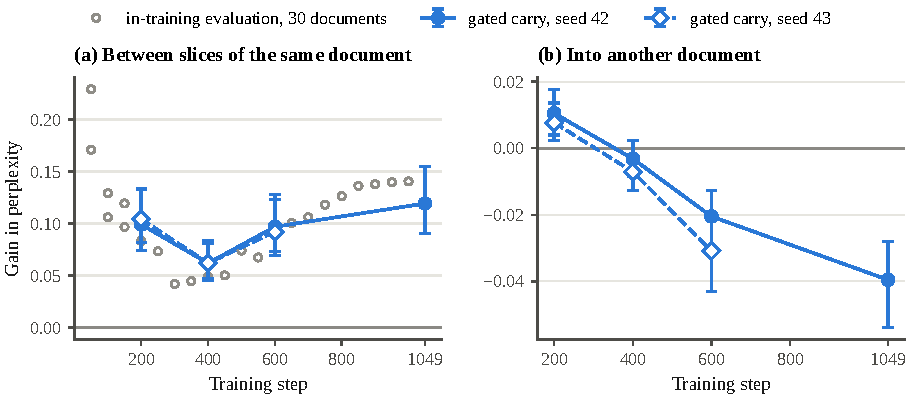
\includegraphics[width=0.95\linewidth]{figures/F15_carry_design_curve.pdf}
    \caption{Gains of the gated carry across training, with 95\% bootstrap intervals, at seed 42 (filled, to step 1049) and seed 43 (open, to step 600). (a) Between slices of the same document, grey circles are in-training evaluations on 30 documents. (b) Into another document of the same source.}
  \label{fig-design}
\end{figure}

Carried into a different document of the same source, the gated carry lowers perplexity by 0.010 $[0.004, 0.018]$ at step 200, but by step 600 it raises it, by 0.020 and 0.031 at the two seeds, and in the run trained to step 1049 by 0.040 $[0.029, 0.054]$. In the boundary suite, the pooled cross-document effect of both ungated runs has an interval including zero at every checkpoint, with intervals about $\pm 0.01$ wide. In the relatedness suite, the Hebbian ungated carry's only measurable effect is a small harm after other-source text ($-0.013$).

\subsection{Ablation}
\label{sec-ablation}

The gated carry combines a separate carry path (A), training through the carry (B) and a nearly closed main gate at the start (C). Table~\ref{tab-ablation} and Figure~\ref{fig-ablation-arch} remove them in turn at step 200. Only the full gated carry recovers the gain between slices, 0.099 and 0.104. Every partial variant stays at or below 0.04. At seed 42 the best partial variant is training through the carry (B, C), with a gain of 0.035, while at seed 43 it is the closed gate alone (C), with 0.040. Therefore, neither component alone accounts for the gain. In single runs that also differed in other settings, training without component C was unstable. But, whether C is needed for the gain is untested. Without it the in-slice Hebbian fast weights raised perplexity to 4703 at step 50, and in a run with neither the zero-initialised scale nor C, the carry gave a perplexity of 31.5 against 16.3 without it at step 100.
\begin{figure}[H]
  \centering
  \begin{minipage}{0.49\linewidth}\centering
    \resizebox{\linewidth}{!}{\ablpanel{0}{0}{(a) Ungated carry, closed gate (C)}{$+0.008$ / $+0.040$}}
  \end{minipage}\hfill
  \begin{minipage}{0.49\linewidth}\centering
    \resizebox{\linewidth}{!}{\ablpanel{1}{0}{(b) Separate path, closed gate (A, C)}{$+0.023$ / $+0.034$}}
  \end{minipage}

  \vspace{6pt}
  \begin{minipage}{0.49\linewidth}\centering
    \resizebox{\linewidth}{!}{\ablpanel{0}{1}{(c) Training through the carry, closed gate (B, C)}{$+0.035$ / $+0.015$}}
  \end{minipage}\hfill
  \begin{minipage}{0.49\linewidth}\centering
    \resizebox{\linewidth}{!}{\ablpanel{1}{1}{(d) Gated carry (A, B, C)}{$+0.099$ / $+0.104$}}
  \end{minipage}
  \caption{Ablation variants at step 200. Crossed-out parts are removed. Gains between slices are given for seeds 42 and 43.}
  \label{fig-ablation-arch}
\end{figure}

\begin{table}[H]
  \centering
  \small
  \begin{tabular}{lrrrr}
    \toprule
    & \multicolumn{2}{c}{Between slices} & \multicolumn{2}{c}{Lead over LoRA-only} \\
    \cmidrule(lr){2-3} \cmidrule(lr){4-5}
    Variant & Seed 42 & Seed 43 & Seed 42 & Seed 43 \\
    \midrule
    Ungated carry, gate bias $-2$ & $+0.014$ & n/a & $+0.073$ & n/a \\
    Ungated carry, closed gate (C) & $+0.008$ & $+0.040$ & $+0.130$ & $+0.117$ \\
    Separate path, closed gate (A, C) & $+0.023$ & $+0.034$ & $+0.172$ & $+0.153$ \\
    Training through the carry, closed gate (B, C) & $+0.035$ & $+0.015$ & $+0.163$ & $+0.179$ \\
    Gated carry (A, B, C) & $+0.099$ & $+0.104$ & $+0.215$ & $+0.214$ \\
    \bottomrule
  \end{tabular}
    \caption{Ablation at step 200, gains in perplexity at two seeds. At seed 42, every 95\% interval excludes zero.}
  \label{tab-ablation}
\end{table}

\subsection{Transfer follows relatedness}
\label{sec-transfer}

On the 200 development cases at step 600, the gated carry lowers perplexity by 0.103 after the target's own first block, by 0.085 after a related article and by 0.051 after an unrelated one, and raises it by 0.067 after text of another source. The other seed reproduces this pattern.

On the 200 confirmatory cases (Figure~\ref{fig-conf}), a related article lowers the target's perplexity by 0.086, while the generic carry lowers it by about 0.07. Therefore, most of the gain after a Wikipedia article is a generic effect of the source. A related article still beats the generic carry by 0.015 and 0.018 (Table~\ref{tab-primary}). Because relatedness is defined by title mentions, this might be due to shared words. On tokens that occur in neither the related nor the random article, a related article still beats a random one (Section~\ref{sec-position}), but we did not run this test against the generic carry. The preregistered decision rules allow the claim of document-specific transfer and of a replicated ordering at both seeds.

In the run trained to the end of the schedule (one seed, retrained separately, not preregistered), the carry is more specific to the document (Tables~\ref{tab-conf} and~\ref{tab-primary}). A related article beats the generic carry by 0.037 and a random article by 0.081, 1.6 to 2.6 times the margins at step 600. We did not test this difference, and it includes variation between runs.

\begin{figure}[H]
  \centering
  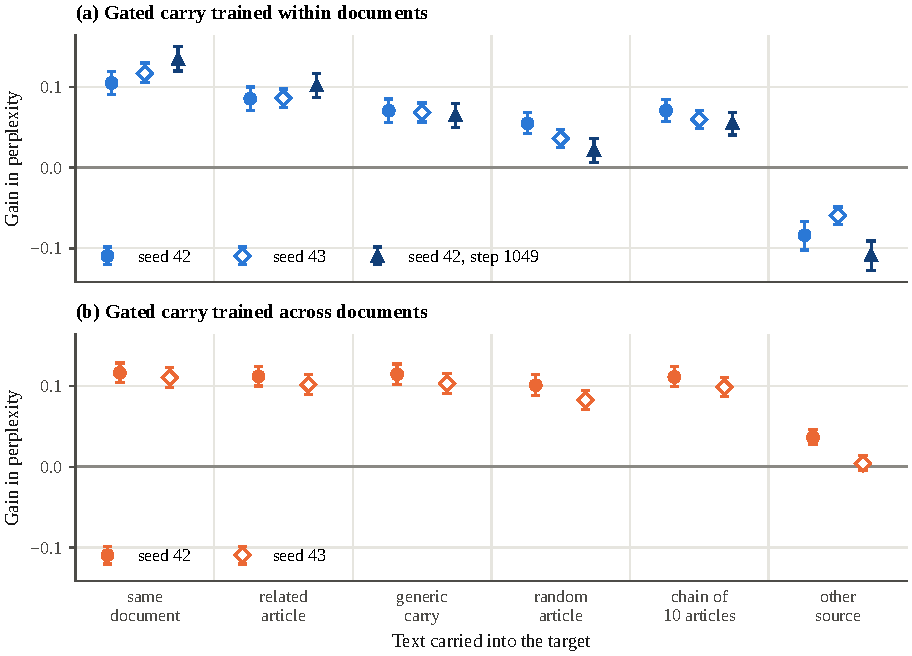
\includegraphics[width=0.85\linewidth]{figures/F18_fresh_relatedness.pdf}
  \caption{Gain in perplexity from the carried text against a reset carry, on 200 preregistered Wikipedia targets, with 95\% bootstrap intervals over targets. (a) The gated carry trained within documents, at seeds 42 and 43 at step 600 and at the end of the schedule. (b) The models trained across documents (Section~\ref{sec-across})}
  \label{fig-conf}
\end{figure}

\begin{table}[H]
  \centering
  \small
  \begin{tabular}{lrrrrr}
    \toprule
    & \multicolumn{3}{c}{Trained within documents} & \multicolumn{2}{c}{Trained across documents} \\
    \cmidrule(lr){2-4} \cmidrule(lr){5-6}
    Carried text & Seed 42 & Seed 43 & Step 1049 & Seed 42 & Seed 43 \\
    \midrule
    Same document & $+0.105$ & $+0.117$ & $+0.135$ & $+0.117$ & $+0.111$ \\
    Related article & $+0.086$ & $+0.086$ & $+0.102$ & $+0.112$ & $+0.102$ \\
    Generic carry & $+0.071$ & $+0.068$ & $+0.065$ & $+0.115$ & $+0.103$ \\
    Random article & $+0.055$ & $+0.036$ & $+0.021$ & $+0.101$ & $+0.083$ \\
    Chain of 10 articles & $+0.071$ & $+0.060$ & $+0.055$ & $+0.111$ & $+0.099$ \\
    Other source & $-0.084$ & $-0.059$ & $-0.109$ & $+0.037$ & $+0.004^{\dagger}$ \\
    \bottomrule
  \end{tabular}
    \caption{Gains from the carry on the 200 confirmatory Wikipedia cases, against a reset carry, at step 600 and, in the Step 1049 column, at step 1049}
  \label{tab-conf}
\end{table}

\begin{table}[H]
  \centering
  \small
  \begin{adjustbox}{max width=\linewidth}
  \begin{tabular}{lrrr}
    \toprule
    Contrast & Seed 42 & Seed 43 & Step 1049 \\
    \midrule
    Same document against generic & $+0.034$ {\footnotesize [$+0.025$, $+0.045$]} & $+0.049$ {\footnotesize [$+0.035$, $+0.064$]} & $+0.070$ {\footnotesize [$+0.052$, $+0.089$]} \\
    Related against generic & $+0.015$ {\footnotesize [$+0.006$, $+0.024$]} & $+0.018$ {\footnotesize [$+0.007$, $+0.029$]} & $+0.037$ {\footnotesize [$+0.021$, $+0.054$]} \\
    Related against random & $+0.031$ {\footnotesize [$+0.016$, $+0.045$]} & $+0.050$ {\footnotesize [$+0.036$, $+0.064$]} & $+0.081$ {\footnotesize [$+0.061$, $+0.102$]} \\
    Carry against in context & $-0.235$ {\footnotesize [$-0.641$, $+0.066$]} & $-0.224$ {\footnotesize [$-0.626$, $+0.076$]} & $-0.209$ {\footnotesize [$-0.611$, $+0.089$]} \\
    \bottomrule
  \end{tabular}
  \end{adjustbox}
    \caption{Preregistered primary contrasts on the confirmatory cases, with Bonferroni-adjusted 98.75\% intervals.}
  \label{tab-primary}
\end{table}

Two results do not fit a simple account. First, in the relatedness suite an unrelated Wikipedia article helps, while in the boundary suite a carry from earlier documents of the same source harms at step 600. Since a chain of ten articles helps more than a chain of one ($+0.017$ and $+0.026$ at the two seeds), accumulation alone does not explain the difference, and by the preregistered rule the conflict remains open. Second, a related article placed in attention has a larger mean gain than the carry but improves only about 45\% of targets, with a median gain of $-0.14$. That condition also moves the scored tokens to later positions. We therefore draw no conclusion from it beyond the preregistered one: the interval of the carry against in context includes zero (Table~\ref{tab-primary}), so that comparison is inconclusive.

\subsection{Where in the target the carry acts}
\label{sec-position}

The gain from a carried text is concentrated at the start of the target (Figure~\ref{fig-position}). At seed 42, 55\% of the gain after the target's own first block and 56\% after a related article fall on the first 31 of 1023 scored tokens, with adjusted intervals of $[48\%, 63\%]$ and $[47\%, 66\%]$, and 54\% and 56\% at seed 43. Over the first seven scored tokens a related article lowers the loss by 0.19 to 0.20 nats per token, after token 128 by 0.001 to 0.002. The harm after other-source text is front-loaded in the same way. This is consistent with the carry acting as a warm start for the opening of a new text. The advantage of a related article over a random one is not confined to tokens that appear in the primes. On the 41\% of target tokens that occur in neither prime it is 0.0022 $[0.0011, 0.0033]$ and 0.0032 $[0.0021, 0.0044]$ nats per token at the two seeds. A generic carry accounts for 66 to 75\% of the related article's gain on the first 31 scored tokens, and the document-specific part, 0.021 $[0.015, 0.028]$ and 0.030 $[0.021, 0.039]$ nats per token, sits there too. After token 128, related and generic differ little. Scored as texts of only 32 tokens, a related article lowers perplexity by 8.0\% and 8.4\% and the generic carry by 6.1\% and 5.6\%, 15 to 18 times the effect on 1024 tokens. These short-text values are reported as a deviation from the preregistration. Its consistency check required them to match the per-token losses within $10^{-3}$ nats, and for every carried text they match only to bfloat16 precision. Addendum B required such a mismatch to be investigated before reporting. The in-context condition does not match and is not reported.

\begin{figure}[H]
  \centering
  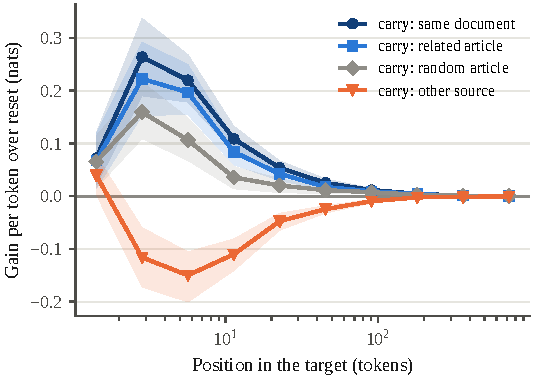
\includegraphics[width=0.65\linewidth]{figures/F19_token_position.pdf}
  \caption{Gain per token from the carried text over a reset carry, by position in the target, for the gated carry at seed 42 on the 200 preregistered cases, with 95\% intervals from resampling clusters of cases.}
  \label{fig-position}
\end{figure}

\subsection{Training across documents}
\label{sec-across}

Against the seed-42 model on the same cases, the probe trained across documents gains 0.120 $[0.103, 0.140]$ more after other-source text, which no longer harms, and 0.041 $[0.028, 0.054]$ more after a chain of ten articles. Its gain after a related article also rises, by 0.027 $[0.013, 0.041]$. However, its carry has become largely generic. A related article does not beat the generic carry ($-0.002$ $[-0.007, +0.003]$), and on the confirmatory holdout the gain between slices of a document falls from 0.125 to 0.073, a change of $-0.052$ $[-0.078, -0.032]$. The probe was not evaluated on the boundary suite. Seed 43 repeats the pattern. In it, other-source text gains 0.064 $[0.051, 0.077]$ more, related against generic is $-0.001$ $[-0.007, +0.004]$, and the gain between slices falls by 0.030 $[0.014, 0.052]$. The seed-42 probe meets the preregistered rule for stating that training across documents removes the harm.

\subsection{What the carried state passes on}

In every model where we measured it, the read-time clip is active on every measurement. In the ungated runs the state exceeds the clip threshold by a factor of at least 255, and in the gated carry by a factor of at least 480, meaning only its direction reaches the output. Reading the same document ten times grows the carried state 3.4-fold. The second reading adds 0.006 and 0.008 at the two seeds, and further readings add nothing measurable. Without the clip, in a single-seed run of 200 steps, the Hebbian model collapsed to a perplexity of about 3300, and in a 100-step run the delta rule trained stably only by closing its gate.

\subsection{Domains}

Within a document the gated carry's between-slice gain has an interval excluding zero on every source at both seeds. Relative to perplexity, it is largest on C4 (1.39\% and 1.46\%), StackExchange (1.35\% and 0.86\%) and Wikipedia (0.99\% and 1.08\%), and smallest on ArXiv, Github and Book (0.18\% to 0.62\%). Across documents of the same source its effect at step 600 is negative on every source, with intervals excluding zero on four sources at seed 42 and on all six at seed 43. For the fast weights within a slice of the ungated carry, the rank correlation between relative gain and base perplexity is weak, 0.20 for the Hebbian rule and 0.09 for the delta rule. With six sources, this cannot show a relation between the difficulty of a source and the gain.

\section{Comparison of Results}
\label{sec-compare}

The gated carry leads the LoRA-only control by 0.234 at step 600, on every document, and by 0.257 and 0.233 on the confirmatory holdout, but most of this lead comes from its 6.7 times larger number of trained parameters. With the same architecture and trainable parameters but no fast-weight updates, the parameter-matched control (seed 42) already leads the LoRA-only control by 0.146 $[0.120, 0.181]$ on the development holdout and 0.158 $[0.125, 0.200]$ on the confirmatory holdout. The gated carry still leads the parameter-matched control, by 0.088 $[0.064, 0.119]$ and 0.068 $[0.047, 0.094]$ at the two seeds on the development holdout and by 0.098 $[0.064, 0.142]$ and 0.075 $[0.046, 0.112]$ on the confirmatory holdout. With its fast weights switched off the gated carry is slightly worse than the control. Therefore, the remaining lead is not explained by the extra parameters, although with one control seed we cannot separate it from variation between runs.

The closest baseline from prior work is dynamic evaluation \citep{krause2018dynamic,krause2019dynamic}, which we apply in a variant on LoRA adapters. We take Adam \citep{kingma2015adam} steps on the LoRA-only model's adapters over the prime and restore them after each case, with the learning rate and number of steps chosen for the related article on 40 separate cases. On the 200 development relatedness cases (not preregistered), it lowers perplexity more than the gated carry after the target's own first block, but less after a related article, and it raises perplexity after a random one. After other-source text it raises perplexity less than the carry ($0.022$ against $0.067$). Each gain is measured against the model's own reset.

Within a document, attention is a far stronger channel when the earlier text is still available. Placing the previous slice of the same document in attention lowers perplexity by 2.770, about 25 times the gated carry's 0.110 on the same tokens (seed 42, development holdout). Also, the carried state, kept in 32-bit precision, takes as much memory as the 16-bit attention cache of about 1500 tokens \citep{ainslie2023gqa,yang2025qwen3}, more than the previous slice used here. Therefore, the carry's possible value lies in use cases where the earlier text is longer than such a cache can hold, or where attention to it is not possible.

% ======================================================================
\chapter{DISCUSSION}

Table~\ref{tab-claims} lists each claim of this report with the evidence behind it and the scope of that evidence.

\begin{table}[H]
  \centering
  \footnotesize
  \begin{tabularx}{\linewidth}{>{\raggedright\arraybackslash}p{4.6cm}>{\raggedright\arraybackslash}X>{\raggedright\arraybackslash}p{2.6cm}}
    \toprule
    Claim & Evidence & Scope \\
    \midrule
    The gated carry lowers perplexity on the continuation of a document by about 1\% & $+0.125$ and $+0.118$ on the confirmatory holdout. $+0.097$ and $+0.092$ on the development holdout & 73 and 106 documents, 2 seeds, earlier slices not in attention \\
    Removing the reset alone gains little & ungated carry at most $+0.040$ within a document at steps 200 to 600. Every pooled cross-document interval of the two ungated runs in the boundary suite includes zero & 24 to 106 documents, 1 seed per rule \\
    Only the combination of the separate path and training through the carry recovers the gain & full design $+0.099$ and $+0.104$. Every partial variant at most $+0.040$ & step 200, 2 seeds \\
    Transfer across documents is ordered by relatedness & same $>$ related $>$ random $>$ other source, every step's interval excludes zero & 200 preregistered cases, 2 seeds, relatedness suite only; the boundary suite differs \\
    A small part of the transfer is document-specific & related against generic $+0.015$ and $+0.018$, Bonferroni-adjusted 98.75\% intervals exclude zero & 200 preregistered cases, 2 seeds \\
    Training across documents removes the harm after other-source text, with no detectable advantage of related text over generic & other source $+0.120$ and $+0.064$ better. Related against generic $-0.002$ and $-0.001$ & 2 seeds (seed 43 not preregistered), 1 mixing ratio, same-source chains not tested \\
    Most of the lead over the LoRA-only control is extra capacity, but the gated carry beats a parameter-matched control & control leads LoRA-only by $+0.146$. Gated carry leads the control by $+0.068$ to $+0.098$ & 73 and 106 documents, 2 gated-carry seeds, 1 control seed \\
    The carry acts mainly on the opening of a new text & 54 to 56\% of the carry's gain on the first 31 of 1023 scored tokens & 200 preregistered cases, 2 seeds, preregistered addendum \\
    At step 1049 the document-specific margins are larger & related against generic $+0.037$, against random $+0.081$ at step 1049 & 200 preregistered cases, 1 separately trained run, not preregistered \\
    \bottomrule
  \end{tabularx}
    \caption{Claims and the evidence for each.}
  \label{tab-claims}
\end{table}

The results separate two questions. Whether a carried fast weight can lower perplexity on later text is answered yes, but substantially only when it is read through its own path and its write is trained for a later read (in the step-200 ablation, 0.099 and 0.104 against at most 0.040). Removing the reset alone results in little gain within a document and nothing measurable across documents in the boundary suite. Whether it then transfers beyond the document depends on relatedness, although in the boundary suite it harms even between documents of the same source. This agrees with work in which related documents in attention help and unrelated ones distract \citep{zhao2024analysing}, training on the nearest neighbours first helps most \citep{hardt2024test}, and a misaligned test-time update can hurt \citep{gandelsman2022ttt}. Interference in shared weights \citep{french1999catastrophic,kirkpatrick2017overcoming} is a natural account of the harm after other-source text, but we did not test it.

The error-correcting write of the delta rule \citep{schlag2021linear,yang2024deltanet} raises the ungated carry's gain only from 0.002 to 0.012 (one seed per rule). Therefore, changing the write rule alone is not enough. In our ablation, the gain appeared only when a separate read path was combined with a training signal for a later read. The gated carry supplies that signal between slices, and the probe supplies it across documents. That the probe removes the harm but loses specificity suggests that a carry harmless at every boundary is easier to learn than one that tells related from unrelated text. The much larger gain from attention matches the finding that full attention outperforms test-time training on long-context recall \citep{tandon2025endtoend}.

\section{Limitations}

We study one model of 0.6 billion parameters with at most two seeds per configuration. The LoRA-only control, the ungated carries and the parameter-matched control have one. Only one gated-carry run, at seed 42, is trained to the end of the schedule, and the other models stop at or before step 600, before the schedule ends. Our intervals cover the sampling of documents, not variation between training runs. The gain within a document is measured with the earlier slices removed from attention. Both models trained across documents use one mixing ratio, the probe was not evaluated on the boundary suite, and the order of the partial ablation variants is not stable across seeds. The relatedness results come from Wikipedia alone, with relatedness defined by title mentions, and this separates topic from shared words only at the level of single tokens. The confirmatory set replicates the relatedness and pooled results, but the boundary, repeat, per-source, ablation and dynamic-evaluation results rest on the development set, which was used to develop the design. The overlap check covers only our training data, not the pretraining data of Qwen3, which likely includes these Wikipedia articles. Also, the confirmatory holdout contains no Book documents, and the difference between the boundary and relatedness suites is unexplained. All evidence is perplexity, which supports claims of stream and domain adaptation but not of memory or recall \citep{song2026beyond}.

% ======================================================================
\chapter{CONCLUSION}

We asked whether the fast weights that test-time training builds while reading one document can usefully be carried into the next. On Q1, removing the reset alone contributes little, at most 0.040 within a document at steps 200 to 600 and nothing measurable across documents in the boundary suite. A gated carry, read through its own path and trained through the boundary between slices, lowers perplexity on the continuation of a document by about 1\% when the earlier text is not in the attention context. Across documents its contribution is small and its sign depends on the relation between the documents. Most of this gain is generic to the source, and a small part depends on the specific relation between the documents. Training across boundaries removes the harm after other-source text but also the advantage of related text over a generic carry, and it lowers the gain within a document. On Q2, within a document on the development holdout, C4, StackExchange and Wikipedia gain most and ArXiv, Github and Book least. Across documents, no source benefits at step 600. For the in-slice gain of the ungated carry, six sources are too few to detect a relation with the difficulty of a source.

\section{Future research}

The direct extensions are more seeds at the full schedule, relatedness measures that separate topic from word overlap in domains beyond Wikipedia, and larger models. The central open question is how a carry trained across documents can keep its advantage on related text. A behavioural test of what the carried state retains, after the earlier text has left the context, is needed before any claim of memory.


\cleardoublepage
\phantomsection
\addcontentsline{toc}{chapter}{References}
\bibliographystyle{plainnat}
\bibliography{references}

\chapter*{Appendix}
\phantomsection
\addcontentsline{toc}{chapter}{Appendix}
\setcounter{section}{0}
\renewcommand{\thesection}{A.\arabic{section}}
\renewcommand{\theHsection}{A.\arabic{section}}
\setcounter{table}{0}
\renewcommand{\thetable}{A.\arabic{table}}

\section{Hyperparameters}
\label{app-hparams}

\begin{table}[H]
  \centering
  \small
  \begin{tabularx}{\linewidth}{>{\raggedright\arraybackslash}p{6.5cm}>{\raggedright\arraybackslash}X}
    \toprule
    Setting & Value \\
    \midrule
    Base model & Qwen3-0.6B \\
    TTT layers (TTT only) & 1, 3, 5, \dots, 27 (14 layers) \\
    Chunk size $C$, fast-weight step $\eta$ (TTT only) & 50, 2 \\
    Target convolution kernel (TTT only) & 8, causal, depthwise \\
    Read-time clip, carried-state decay (TTT only) & 20, 0.9 \\
    Main gate bias at initialisation & $-6$ gated carry, $-2$ ungated carry ($-6$ in ablation C) \\
    Carry path & separate gate, scale $\alpha$ initialised to 0 \\
    Training through the carry & window of 2 slices \\
    LoRA rank, scaling, dropout & 16, 32, 0.05 \\
    Learning rates, LoRA, down-projection, new modules & $10^{-5}$, $3 \times 10^{-5}$, $6 \times 10^{-2}$ \\
    Gradient clip, accumulation, warmup & 10, 16, 2\% of steps \\
    Schedule & cosine over 1050 steps (1048 for seed 43) \\
    Training documents & 4000, 2048 to 16{,}384 tokens \\
    Seed & 42, and 43 for the second gated-carry run, the ablations and the probe \\
    Parameter-matched control & gated-carry architecture, fast-weight updates disabled \\
    Probe trained across documents & sessions of 5 documents, same source with probability 0.5 \\
    Bootstrap resamples & 1000, and 10{,}000 on the confirmatory set \\
    \bottomrule
  \end{tabularx}
  \caption{Training and evaluation settings. TTT only marks settings that apply only to models with TTT layers.}
\end{table}

\end{document}
